\section{Gaussian Channels with Feedback}
Recalling the fact that, Capacity doesnot change with adding Feedback to DMC (Discrete MemoryLess Channels), and the same holds true for an additive noise channel but having a Feedback can surely reduce the encoding and decoding complexity.When it comes to Channels with Memory, from time to time the noise gets correlated.Though Capacity without Feedback can be easily calculated using the $"Water - Fillng"$ process, same cannot be said for Gaussian Channels with Feedback.
The Capacity of Gaussian Channels with Feedback can be derived by the noise $\mathbf{Z}$  covariance matrix.
%%%%%%%%%%%%%%%%%%%%%%%%%%%%%
 %%We prove a converse for this expression, which then derives a simple bound on the increase in capacity due to feedback.%%
%%%%%%%%%%%%%%%%%%%%%%%%%%%%%
\\
The Gaussian channel with feedback can be seen as below ,
\begin{center}
	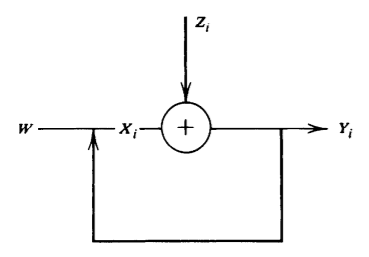
\includegraphics[scale=0.5]{Diagrams/Gaussian_Channel_with_FeedBack.png}
\end{center} 
 $Y_i$ which is the output of the channel is given by,
\begin{equation}
Y_i = X_i + Z_i, \quad Z_i \sim \mathcal{N}(0, K_Z^{(i)}). \label{eq:10.96}
\end{equation}
Hence , it is clear that the input of the channel depends on the past values of the output due to concept of Feedback.
%
\begin{tcolorbox}[boxrule=0pt,frame hidden,sharp corners,enhanced, opacityback=0, borderline west={2pt}{0pt}{red}]
\begin{defn} \textbf{(Gaussian Channel with Feedback)}
Gaussian channel with feedback with $(2^{nR}, n)$ code and consisting sequences of input message which is $x_i(W, Y^{i-1})$, where $W \in \{1, 2, \dots, 2^{nR}\}$ and the value coming from output due to Feedback is described $Y^{i-1}$. 
$\mathbf{x}(W, \cdot)$ can be considered as a code function and it has to satisfy the power constraint,
\begin{equation}
E\left[\frac{1}{n} \sum_{i=1}^n x_i^2(W, Y^{i-1})\right] \leq P, \quad w \in \{1, 2, \dots, 2^{nR}\}, \label{eq:10.97}
\end{equation}
Where the equation covers all noise sequence possibilities.
Since a Feedback Path is involved ,$X_i$ is dependent causally on the past values of ${Z}$.
\end{defn}
\end{tcolorbox}
%
\subsection{Without feedback}
Considering a time-varying Gaussian Channel without Feedback , whose Capacity is described by
\begin{equation}
C_{n} = \max_{\frac{1}{n}\text{tr}(\mathbf{K}_X^{(n)}) \leq P} \frac{1}{2n} \log \frac{|\mathbf{K}^{(n)}_{X}+ {K}^{(n)}_{Z}|}{|\mathbf{K}^{(n)}_Z|}
\end{equation}
%
on Eigenvalues ${\lambda_i^{(n)}}$ of $\mathbf{K}_Z^{(n)}$, applying Water-Filling we get:
\begin{equation}
C_n = \frac{1}{2n} \sum_{i=1}^n \log \left(1 + \frac{(\lambda - {\lambda_i^{(n)}})^+}{\lambda_i^{(n)}} \right)
\end{equation}
where $(y)^+ = \max(y, 0)$ 
\\
and $\lambda$ has to be chosen such that $\sum_{i=1}^n (\nu - \lambda_i^{(n)})^+ = nP$

Considering a Gaussian Channel with Feedback
We now state an informal characterization of the capacity of the channel with and without feedback.

\subsection{With feedback}
Considering a time-varying Gaussian Channel with Feedback , whose Capacity in bits per transmission is described by
\begin{equation}
C_{n,FB} = \max_{\frac{1}{n}\text{tr}(\mathbf{K}_X^{(n)}) \leq P} \frac{1}{2n} \log \frac{|\mathbf{K}^{(n)}_{X+Z}|}{|\mathbf{K}^{(n)}_Z|}
\tag{5.1}
\end{equation}
\newpage
$X^n$ maximization without any loss of generality is of the form:
\begin{equation}
X_i = \sum_{j=1}^{i-1} b_{ij}Z_j + V_i, \quad i=1,2,\dots,n 
\tag{5.2}
\end{equation}
where above $V^n$ is independent of $Z^n$.
\\
$X^n$ $+$ $Z^n$ distribution achieving the maximum entropy is Gaussian. Jointly Gaussian Distribution $(X^n, Z^n,X^n+ Z^n)$ achieves maximization since $Z^n$ is also Gaussian.
Since, $Z^n$ $=$ $Y^n$ $-$ $X^n$ dependent on $Y^n$ , $X^n$ of the above form $eq $ $5.2$.
 using $X = {BZ} + {V}$ and ${Y} = {X} + {Z}$, rewriting $eq $ $5.1$ as:
\begin{equation}
C_{n,FB} = \max \frac{1}{2n} \log  \frac{|(\mathbf{B+I})(\mathbf{K^{(n)}_Z})(\mathbf{B+I})^t+\mathbf{K_v}|}{|\mathbf{K^{(n)}_Z|}}  \label{eq:10.100}
\end{equation}
where the maximum is taken over all positive definite ${K_v}$, and lower triangular ${B}$ such that
\begin{equation}
tr(\mathbf{B}\mathbf{K^{(n)}_Z}\mathbf{B}^t + \mathbf{K}_V) \leq nP. \label{eq:10.101}
\end{equation}
${B}$ becomes $0$ when there is no Feedback.

%
\begin{tcolorbox}[boxrule=0pt,frame hidden,sharp corners,enhanced, opacityback=0, borderline west={2pt}{0pt}{blue}]
\textbf{Theorem 10.6.1:} Tor the Gaussian channel with feedback with code $(2^{nR}, n)$, the rate $R_n$  with $P_e^{(n)} \to 0$  satisfies
\begin{equation}
R_n = \frac{1}{n} \left( \frac{1}{2} \log \left| \frac{\mathbf{K}_Y^{(n)}}{\mathbf{K}_Z^{(n)}} \right| + \epsilon_n \right) \label{eq:10.105}
\end{equation}
with $\epsilon_n \to 0$ as $n \to \infty$.
\end{tcolorbox}
%
\textit{Proof:} 
\\
\begin{tcolorbox}[boxrule=0pt,frame hidden,sharp corners,enhanced, opacityback=0, borderline west={2pt}{0pt}{red}]
\begin{defn} \textbf{Fano's Inequality} 
\begin{equation}
H(W|Y^n) \le 1 + nR_n P_e^{(n)} = n\epsilon_n \label{eq:10.106}
\end{equation}
where $\epsilon_n \to 0$ as $P_e^{(n)} \to 0$
\end{defn}
\end{tcolorbox}
%
Using Fano's Inequality , Rate can be bounded as:
\begin{align}
nR_n &= H(W)  \\
\end{align}
By relation between Entropy and Mutual Information, it can be written as 
\begin{align}
nR_n = I(W;Y^n) + H(W|Y^n)  \\
\end{align}
and it can be also written as ,
\begin{align}
nR_n \le I(W;Y^n) + \epsilon_n  \\
\end{align}
By Properties of Mutual Information we get,
\begin{align}
nR_n = \sum_i I(W;Y_i|Y^{i-1}) + \epsilon_n  \\
\end{align}
By relation between Entropy and Mutual Information, it can again be written as 
\begin{align}
(a)&= \sum_i h(Y_i|Y^{i-1}) - h(Z_i|W,Y^{i-1},X_i,X^{i-1},Z^{i-1}) + \epsilon_n  \\
\end{align}
\newpage
 Since , $X_i$ is a function of $W$ and the past $Y^{i-1}$, and $Z^{i-1}$ is $Y^{i-1} - X^{i-1}$.
\begin{align}
(b)&= \sum_i h(Y_i|Y^{i-1}) - h(Z_i|W,Y^{i-1},X_i,X^{i-1},Z^{i-1}) + \epsilon_n  \\
\end{align}
Since, $Y_i = X_i + Z_i$ and the fact that $h(X + Z|X) = h(Z)$
\begin{align}
(c)&= \sum_i h(Y_i|Y^{i-1}) - h(Z_i|Z^{i-1}) + \epsilon_n  \\
\end{align}
Since, $(W,Y^{i-1},X^i)$ are conditionally independent given $Z^{i-1}$
\begin{align}
nR_n= h(Y^n) - h(Z^n) + n\epsilon_n \\
\end{align}
Diving the above equation  by $n$ and Continuing the chain of inequalities the entropy maximizing property ,
\begin{equation}
R_n \le \frac{1}{n} [h(Y^n) - h(Z^n)] + \epsilon_n \le \frac{1}{2n} \log \left| \frac{\mathbf{K}_Y^{(n)}}{\mathbf{K}_Z^{(n)}} \right| + \epsilon_n, \label{eq:10.115}
\end{equation}
For Gaussian channel with feedback, the above is the upper bound on the capacity. 
\\
\begin{tcolorbox}[boxrule=0pt,frame hidden,sharp corners,enhanced, opacityback=0, borderline west={2pt}{0pt}{blue}]
\textbf{Lemma :} Let $\mathbf{X}$ and $\mathbf{Z}$ be $n$-dimensional random vectors. Then
\begin{equation}
\mathbf{K}_{X+Z} + \mathbf{K}_{X-Z} = 2\mathbf{K}_X + 2\mathbf{K}_Z \label{eq:10.116}
\end{equation}
\end{tcolorbox}
\textit{Proof:}
${K}_{X+Z}$ can be written as the following in terms of expectation:
\begin{align}
\mathbf{K}_{X+Z} &= E[\mathbf{(X + Z)(X + Z)}^\top] \\
\end{align}
by expanding all terms , we get
\begin{align}
\mathbf{K}_{X+Z} &=E[\mathbf{XX}^\top + \mathbf{XZ}^\top + \mathbf{ZX}^\top + \mathbf{ZZ}^\top]  \\
&= \mathbf{K}_X + \mathbf{K}_{XZ} + \mathbf{K}_{ZX} + \mathbf{K}_Z\\
\end{align}
When done the same for ${K}_{X-Z}$ , we get
\begin{equation}
\mathbf{K}_{X-Z} = \mathbf{K}_X - \mathbf{K}_{XZ} - \mathbf{K}_{ZX} + \mathbf{K}_Z \label{eq:10.120}
\end{equation}
Adding the above final equations we get,
\begin{equation}
\mathbf{K}_{X+Z} + \mathbf{K}_{X-Z} = 2\mathbf{K}_X + 2\mathbf{K}_Z \label{eq:10.116}
\end{equation}

\begin{tcolorbox}[boxrule=0pt,frame hidden,sharp corners,enhanced, opacityback=0, borderline west={2pt}{0pt}{blue}]
\textbf{Lemma :} For two $n \times n$ non-negative definite matrices $\mathbf{A}$ and $\mathbf{B}$, if $\mathbf{A} - \mathbf{B}$ is non-negative, then $|\mathbf{A}| \ge |\mathbf{B}|$.
\end{tcolorbox}
\textit{Proof:} Let $\mathbf{C} = \mathbf{A} - \mathbf{B}$  and both $\mathbf{B}$ and $\mathbf{C}$ are non-negative considering them as covariance matrices.
Let $\mathbf{X}_1 \sim \mathcal{N}(\mathbf{0}, \mathbf{B})$ and $\mathbf{X}_2 \sim \mathcal{N}(\mathbf{0}, \mathbf{C})$ two independent normal random vectors and $\mathbf{Y} = \mathbf{X}_1 + \mathbf{X}_2$. 
Then by properties of Entropy,
\begin{equation}
h(\mathbf{Y}) \ge h(\mathbf{Y}|\mathbf{X}_2) \label{eq:10.121}
\end{equation}
Since conditioning reduces differential entropy and the above can also be written as,
\begin{equation}
= h(\mathbf{X}_1|\mathbf{X}_2) \label{eq:10.122}
\end{equation}
Since  $\mathbf{X}_1 $, $ \mathbf{X}_2$ are independent of each other.
\begin{equation}
= h(\mathbf{X}_1) \label{eq:10.123}
\end{equation}
\newpage
Substituting the above in the formula for differential entropies of a normal random variable,
\begin{equation}
\frac{1}{2} \log(2\pi e){|A|} \geq \frac{1}{2} \log(2\pi e){|B|}, \label{eq:10.124}
\end{equation}

and canceling  common terms, we get $|\mathbf{A}| \ge |\mathbf{B}|$

\begin{tcolorbox}[boxrule=0pt,frame hidden,sharp corners,enhanced, opacityback=0, borderline west={2pt}{0pt}{blue}]
\textbf{Lemma :} For two $n$-dimensional random vectors $\mathbf{X}$ and $\mathbf{Z}$,
\begin{equation}
|\mathbf{K}_{\mathbf{X}+\mathbf{Z}}| \le 2^{n}|\mathbf{K}_\mathbf{X}+\mathbf{K}_\mathbf{Z}| 
\end{equation}
\end{tcolorbox}
\textit{Proof:} From 1st Lemma,
\begin{equation}
2(\mathbf{K}_\mathbf{X} + \mathbf{K}_\mathbf{Z}) - \mathbf{K}_{\mathbf{X}+\mathbf{Z}} - \mathbf{K}_{\mathbf{X}-\mathbf{Z}} \ge 0, \label{eq:10.126}
\end{equation}
where $\mathbf{A} \ge 0$ ,upon applying 2nd Lemma , we have
\begin{equation}
|\mathbf{K}_{\mathbf{X}+\mathbf{Z}}| \le |2(\mathbf{K}_\mathbf{X}+\mathbf{K}_\mathbf{Z})|= 2^{n}|\mathbf{K}_\mathbf{X}+\mathbf{K}_\mathbf{Z}|
\end{equation}

\begin{tcolorbox}[boxrule=0pt,frame hidden,sharp corners,enhanced, opacityback=0, borderline west={2pt}{0pt}{blue}]
\textbf{Theorem 10.6.2:}
\begin{equation}
C_{n,FB} \leq C_n + \frac{1}{2} \text{ bits per transmission} \label{eq:10.128}
\end{equation}
\end{tcolorbox}
\textit{Proof:} Combining all the 3 proved lemmas, we obtain
\begin{align}
C_{n,FB} &\leq \max_{\text{tr}(\mathbf{K}_\mathbf{X})\leq nP} \frac{1}{2n} \log \left| \frac{\mathbf{K_Y}}{\mathbf{K_Z}} \right|  \\
&\leq \max_{\text{tr}(\mathbf{K}_\mathbf{X}) \leq nP} \frac{1}{2n} \log  \frac{2^{n}|\mathbf{K}_\mathbf{X} + \mathbf{K}_\mathbf{Z}|}{|\mathbf{K}_\mathbf{Z}|} \\
&=\max_{\text{tr}(\mathbf{K}_\mathbf{X}) \leq nP} \frac{1}{2n} \log  \frac{|\mathbf{K}_\mathbf{X} + \mathbf{K}_\mathbf{Z}|}{|\mathbf{K}_\mathbf{Z}|} + \frac{1}{2}\\
&\leq C_n + \frac{1}{2} \text{ bits per transmission}, \label{eq:10.132}
\end{align}
The above proves in a non-white Gaussian additive noise channel feedback increases the capacity by at most half a bit.





